\documentclass{article}
\usepackage{graphicx}
\usepackage{amsmath}
\usepackage{hyperref}
\usepackage{amsmath}
\usepackage{amsfonts}
\usepackage{parskip}
\usepackage{cleveref}
\usepackage{xcolor} 
\setlength{\parindent}{0em}
\usepackage[margin=1.0in]{geometry}
\begin{document}

\begin{flushleft}
    \textbf{\large{Problem Set \#3}} \\
    MACSS 3000, Prof. Evans \\
    Benjamin Rothschild
\end{flushleft}

\section*{Problem 1}
\subsection*{Part A}
\begin{center}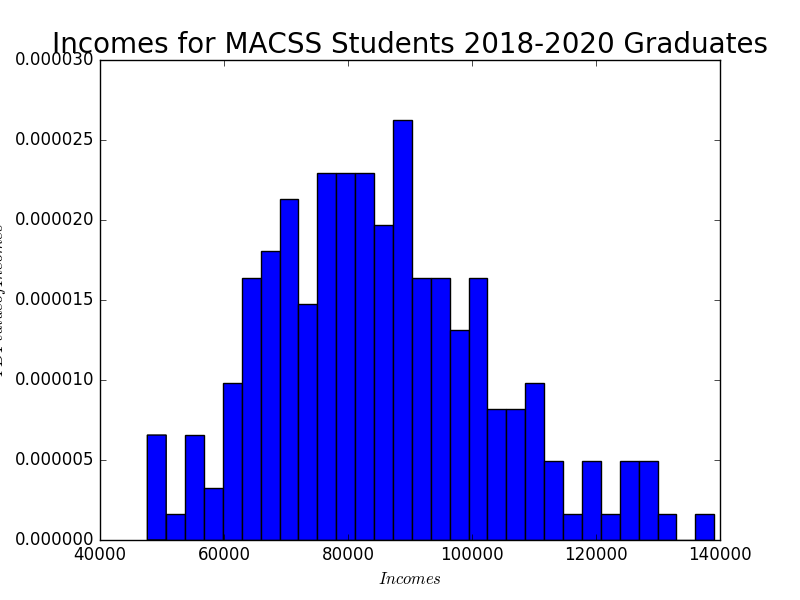
\includegraphics[width=100mm]{images/1a.png}\end{center}

\subsection*{Part B}
Using the average income and std dev of income as my moments I got the following model.  $\mu$ = 11.3369, $\sigma$ = 0.2130.  The value of the criterion func is 3.69767244327e-12.  The comparision for my model moments vs the data moments are below.  The modeled values are very close to the data values.

\begin{center}
  \begin{tabular}{ l | c | c }
    \hline
     & model & data \\ \hline
    mean & 85276.6695 & 85276.8236 \\ \hline
    std & 17992.5303 & 17992.5421 \\
    \hline
  \end{tabular}
\end{center}
\begin{center}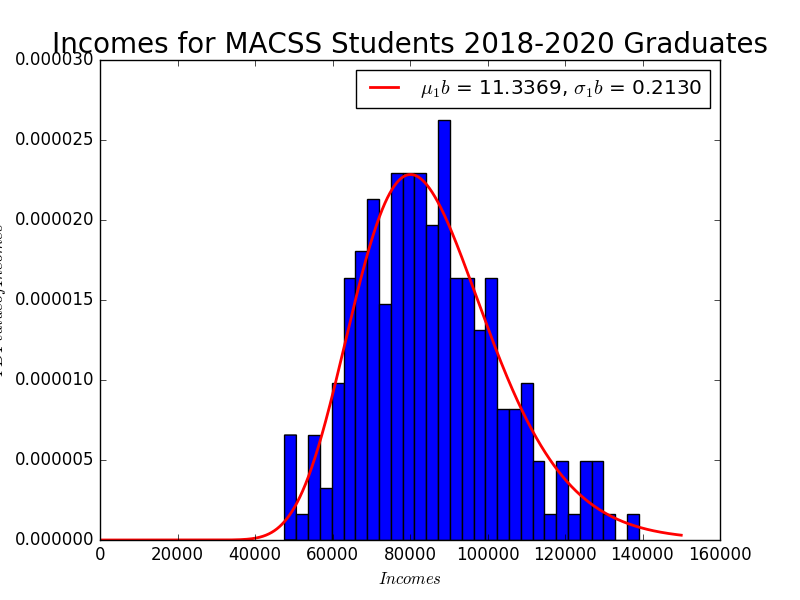
\includegraphics[width=100mm]{images/1b.png}\end{center}

\subsection*{Part C}
Using the average income and std dev of income as my moments and the variance covariance matrix I got the following model.  $\mu$ = 11.1254, $\sigma$ = 0.5259.  The value of the criterion func is 0.000172573277268.  The comparision for my model moments vs the data moments are below and as can be seen in the graph the model is not a great fit for the data.
\begin{center}
  \begin{tabular}{ l | c | c }
    \hline
     & model & data \\ \hline
    mean & 65230.7802 & 85276.8236 \\ \hline
    std & 29635.6986 & 17992.5421 \\
    \hline
  \end{tabular}
\end{center}
\begin{center}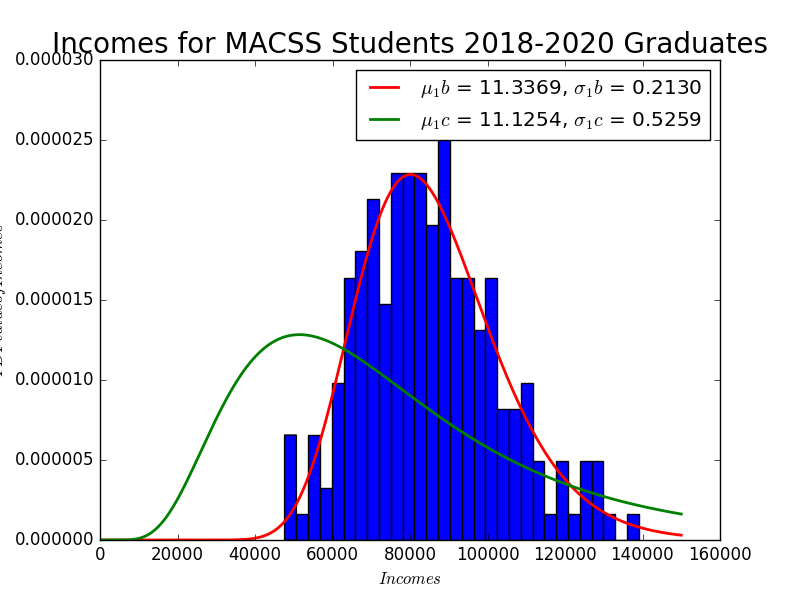
\includegraphics[width=100mm]{images/1c.png}\end{center}


\subsection*{Part D}
Using the three specified moments I got the following model $\mu$ = 11.336, $\sigma$ = 0.211.  The value of the criterion func is 2.50777261786e-11.  The comparision for my model moments vs the data moments are:

\begin{center}
  \begin{tabular}{ l | c | c }
    \hline
     & model & data \\ \hline
    moment 1 & 0.3 & 0.3 \\ \hline
    moment 2 & 0.5 & 0.5 \\ \hline
    moment 3 & 0.2 & 0.2 \\
    \hline
  \end{tabular}
\end{center}
\begin{center}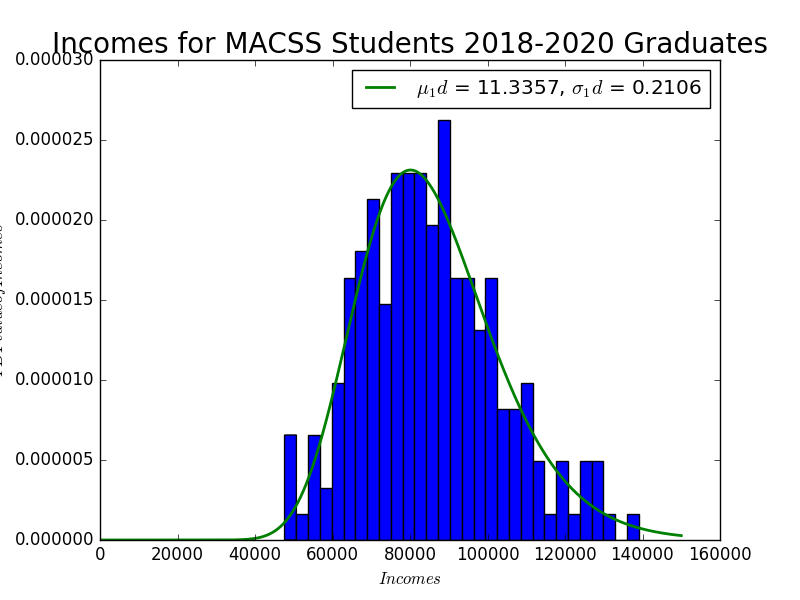
\includegraphics[width=100mm]{images/1d.png}\end{center}



\subsection*{Part E}
Using the three specified moments and the variance covariance matrix I got the following model.  $\mu$ = 11.336, $\sigma$ = 0.213.  The value of the criterion func is 1.23151119235e-10.  The comparision for my model moments vs the data moments are below.  The results are very similar to Part D.

\begin{center}
  \begin{tabular}{ l | c | c }
    \hline
     & model & data \\ \hline
    moment 1 & 0.3 & 0.301 \\ \hline
    moment 2 & 0.5 & 0.495 \\ \hline
    moment 3 & 0.2 & 0.204 \\
    \hline
  \end{tabular}
\end{center}
\begin{center}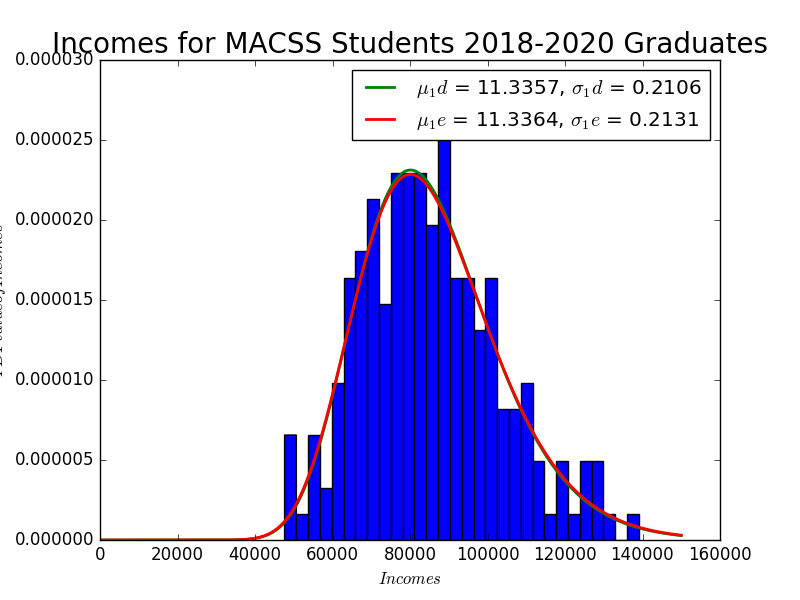
\includegraphics[width=100mm]{images/1e.png}\end{center}

\subsection*{Part F}
In the analysis I used four different methods for modeling the incomes data.  I got good results by using the GMM on mean and std deviation as well as using GMM on the three moments given in the problem set.  This can be seen by comparing the graphs of the modeled $\mu$ and $\sigma$ as well as looking at the criterion function values.  The criterion function returns an error value and as can be seen in part B, D, and E the value is very small.  I don't know if I could say one of these models is more accurate than the other as they precision of the criterion value is very small and close to each other.
\section*{Problem 2}

\subsection*{Part A}
My paramter estimates from GMM are $\beta_0$=0.25164544, $\beta_1$=0.01293354, $\beta_2$=0.4005004, $\beta_3$=-0.00999177.  The criterion value is = 0.0018212898086065973.

\end{document}